\documentclass[a4paper]{extarticle}
\usepackage[utf8]{inputenc}
\usepackage[a4paper, margin=1in]{geometry}

\usepackage{amssymb}
\usepackage{amsmath}
\usepackage{enumitem}
\usepackage{tcolorbox}
\usepackage{fancyhdr}
\usepackage{graphicx}
\usepackage{float}

\setlength{\parindent}{0em}
\setlength{\parskip}{0.4em}

\definecolor{theoremblue}{RGB}{1, 73, 124}
\definecolor{corollaryblue}{RGB}{70, 143, 175}
\definecolor{exampleblue}{RGB}{137, 194, 217}

\newtcolorbox{tbox}{colback=theoremblue!20,colframe=theoremblue,
boxrule=0pt,arc=0pt,boxsep=2pt,left=2pt,right=2pt,leftrule=2pt}

\newtcolorbox{cbox}{colback=corollaryblue!20,colframe=corollaryblue,
boxrule=0pt,arc=0pt,boxsep=2pt,left=2pt,right=2pt,leftrule=2pt}

\newtcolorbox{ebox}{colback=exampleblue!20,colframe=exampleblue,
boxrule=0pt,arc=0pt,boxsep=2pt,left=2pt,right=2pt,leftrule=2pt}

\title{EnpRisk - Lecture Notes Week 12}
\author{Ruben Schenk, ruben.schenk@inf.ethz.ch}
\date{\today}

\pagestyle{fancy}
\fancyhf{}
\rhead{ruben.schenk@inf.ethz.ch}
\rfoot{Page \thepage}
\lhead{EnpRisk - Lecture Notes Week 12}

\begin{document}

\maketitle

\section{Financial Stability and Entrepreneurial Risk}

The link between financial stability and business development is because we believe that financial stability is a precondition for sustainable economic growth.

A stable and well-functioning financial system exists to serve us all. It enables the efficient allocation of resources, so that businesses can exploit productive opportunities and households can meet their needs. It allows the risks incurred in the course of generating economic growth to be shared.

Macro-prudential policy should be targeted to provide a net benefit to the overall economy.

\subsection{Where does money come from?}

Many people think of money as a special thing that has value because it is scarce or because everyone believes in it.

Money is a financial claim, backed by debt! Banks do not store money. Desposits are a bank's liability backed by (risky) long-term assets.

\begin{figure}[H]
    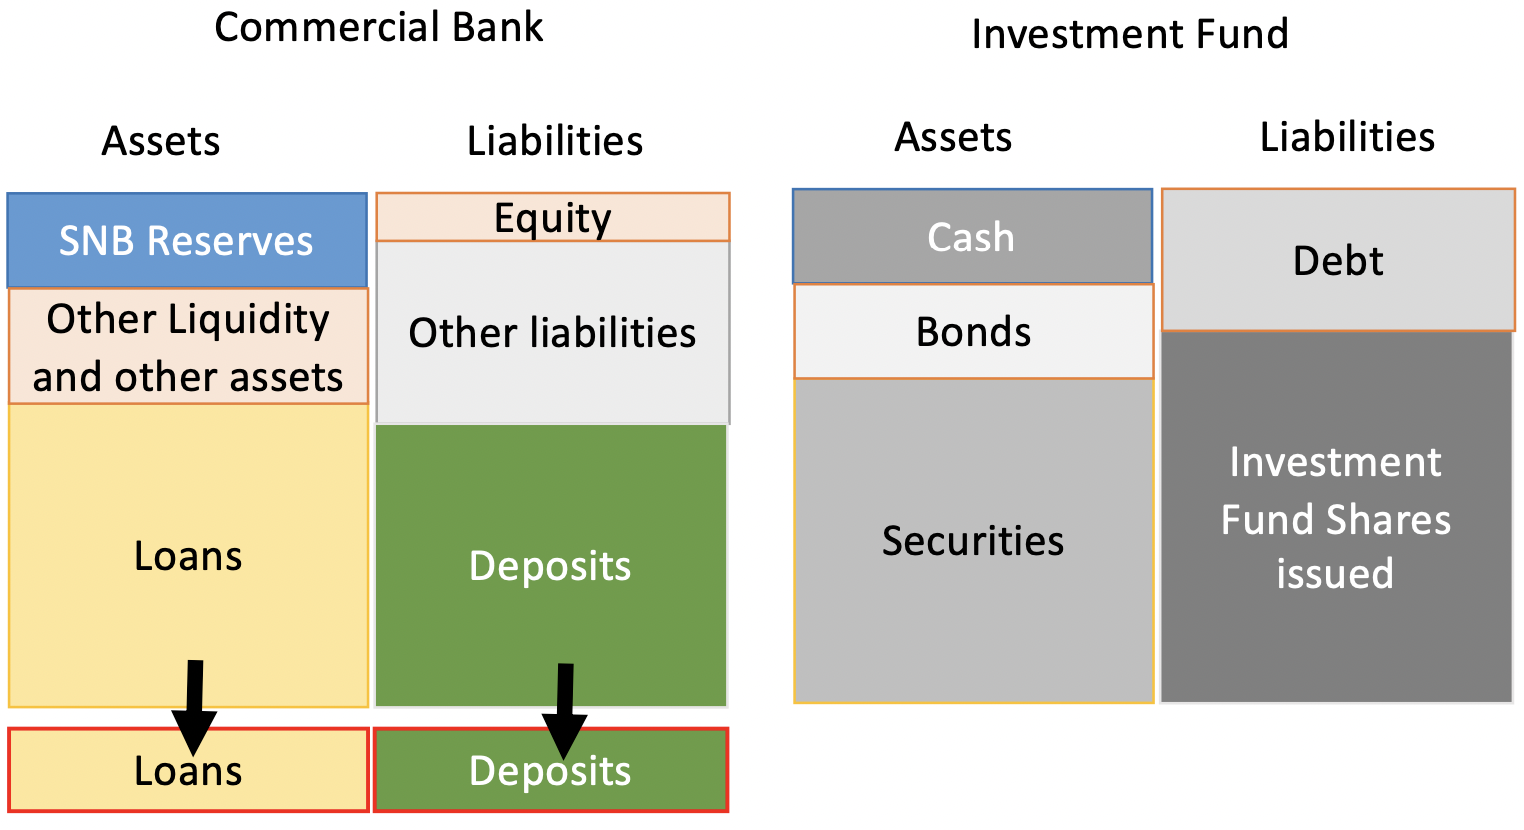
\includegraphics[width=15cm]{../images/EnpRisk_Fig12-1}
    \centering
\end{figure}

It is essential to know exactly in which legal form your assets are held to be able to asses the risks of losing all or part of it. Example: In th event of bankruptcy, crypto assets held by the exchange could be considered property of the bankruptcy proceedings and customers could be treated as unsecure creditors. An unsecure creditor would be one of the last to be paid in any bankrutcy and last in line for claims.

Three principles to answer almost any macrofinancial question:

\paragraph{For every financial debt, there is a financial assets} The sum over all financial assets and liability is always zero. The sum of real assets (machines etc.) can be positive.

\paragraph{Follow the money} Money creation for consumption or certain government spending can increase inflation (consumer price index). Money creation for speculative financial activities can drive asset prices temporarily while leaving the consumer prices largely unaffected.

\paragraph{Look at the system as a whole} Not everyone can save. Companies, households and the state can only be net savers in Switzerland (in the financial sense) because foreign countries are in debt.

\subsection{How the financial system has changed over the last decades}

\subsubsection{Great Mortgaging}

Following some motivation do disaggregate credit:

\begin{itemize}
    \item Economic development/growth: Neither consumption credit nor household mortage are directly linked to productivity growth in the way that loans to non-financial firms are. Empirical financial-development literature often englected diaggregation of credit.
    \item Inequality in wealth and income: Growth of bank credit can reduce income inequality if reducing investment barriers. In advacned economies, fiancialization/growth of Finance, Insurance and Real Estate (FIRE) sector and lending to asset markets can increase inequalities.
    \item Financial stability: Conditional on having a recession, stronger credit growth predicts deeper recessions. Household credit increases probability of crisis.
\end{itemize}

In Switzerland, 90\% of loans are mortgages, i.e. secured by real estate. Yet textbooks typically say that banks examine and pool the risk of entrepreneurs' business models. Globally, the volume of mortgages is also growing strongly compared to GDP, while non-mortgage corporate loans are growing less strongly.

In advanced economies (AEs), increase in mortage creadit has positive effect on business credit in short-run, and less significant negative effect in medium-run. Increase in mortage credit has a negative effect on GDP. Firm investment in intangible assets increases, therefore banks might reallocate towards real estate and liquid assets.

\subsubsection{Rise of Non-banks}

The \textbf{non-bank financial intermediation (NBFI)} sector is a broad measure of all non-bank financial entities, composed of all financial institutions that are non central banks, banks or public financial institutions. Originally, they were called \textit{shadow banks} to describe borrowing and lending outside the regulated banking system.

NBFI assets increased over the last 20 years. They mainly consist of pension funds, investment funds, money market funds, insurance corporations etc.

An example is the American International Group (AIG) which in 2007 looked more like a bank than like an insurance firm, and almost failed as a result of two large bets on real estate:

\begin{enumerate}
    \item AIG life insurence lends out ehr assets against cash (security lending), and invests the cast in risky assets linked to real estate. The security borrower can give the assets back and claim the cash within 1 day!
    \item AIG sold insurance on real-estate-abcked derivatives.
\end{enumerate}

AIG's reliability became more "bank-like" and subject to rollover risk at the same time that its assets became more opaque and iliquid, and again more bank-like, increasing its vulnerability to a shock.

Can pension funds increase or trigger instability? In theory, asset allocation of PFs can contribute to asset bubbles and the failure of PFs to pay pensioners could for example trigger isntability via lowering household income and associate loan-to-income ratios. The empiric view is shown in the following table:

\begin{figure}[H]
    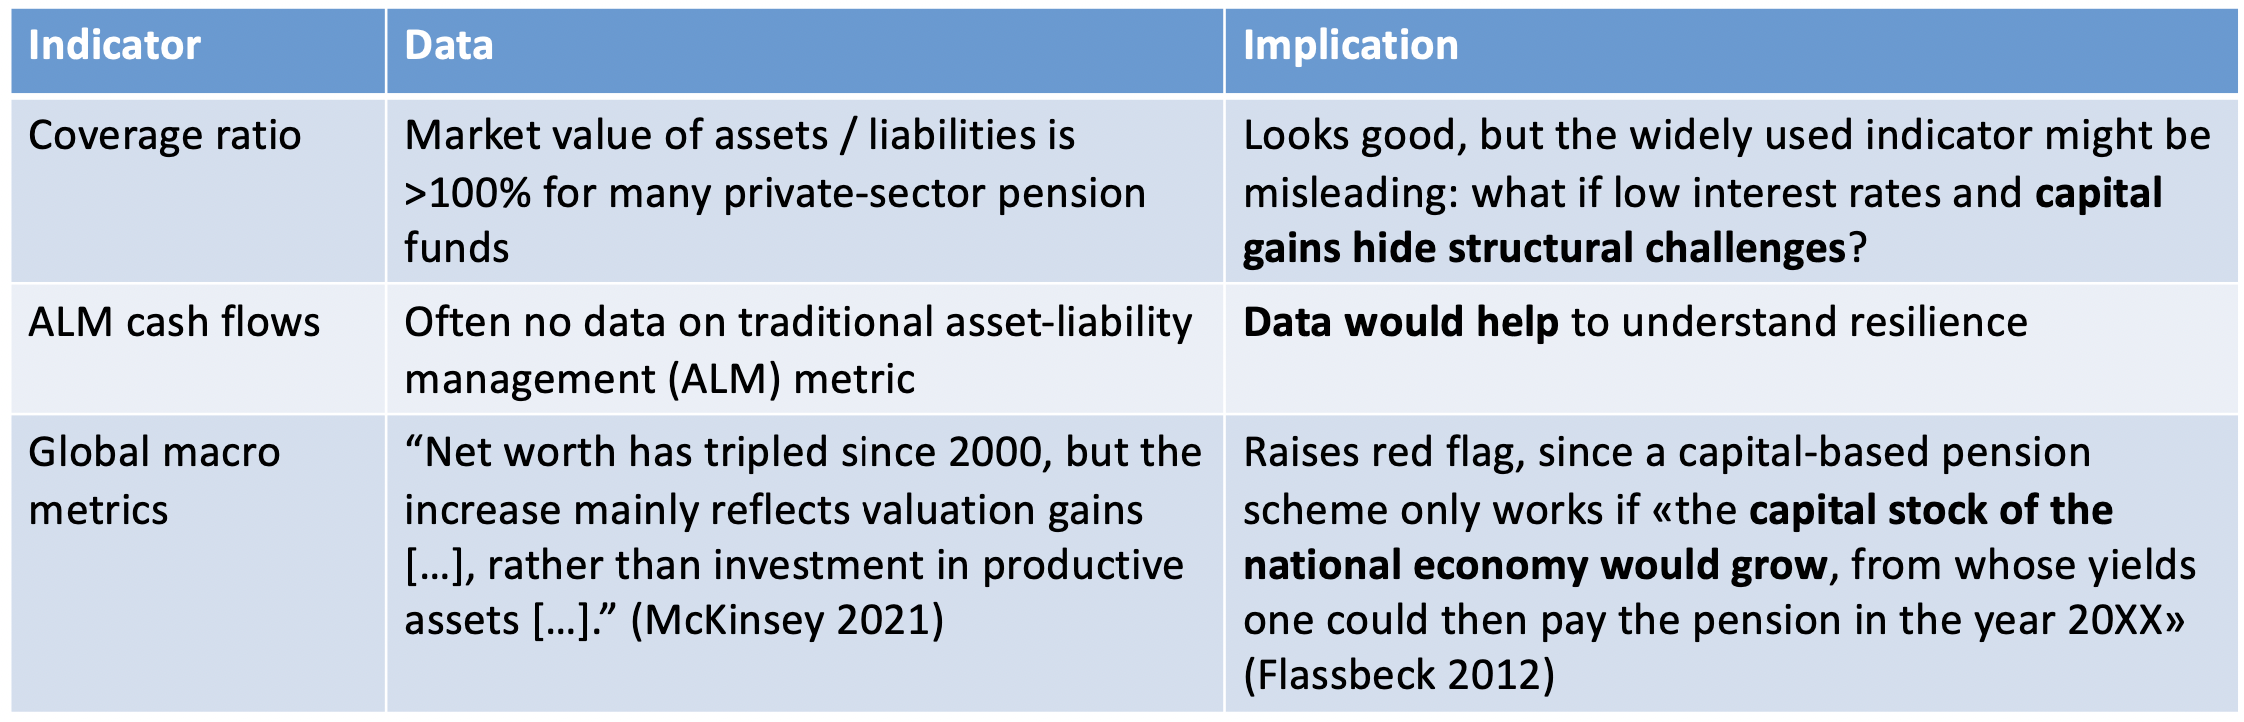
\includegraphics[width=15cm]{../images/EnpRisk_Fig12-2}
    \centering
\end{figure}

\subsection{Fit for purpose or zero risk society?}


\end{document}